%%
%% Author: Gerard Bosch (gerard.bosch@gmail.com)
%% 13/02/2018
%%

\documentclass[notitlepage, usenames,dvipsnames]{beamer}
\usefonttheme[onlymath]{serif}      %font serif (beamer usa sans-serif) per a l'entorn math

\usepackage{beamerprosper}
%\usepackage{pstricks-add}
%\usepackage{beamertexpower}
\usepackage[utf8]{inputenc}
\usepackage[english]{babel}
%\usepackage{default}
\usepackage{verbatim}
\usepackage{multicol}
\usepackage{graphicx}
\usepackage{comment}
%\usepackage{pgfpages}

%\setbeameroption{show notes on second screen=right}    % pgfpages package
\setbeamertemplate{navigation symbols}{}

%% Aliases %%
\renewcommand{\tt}{\texttt}     %redefinit! és l'entorn typewriter, però sempre faig anar verbatims.
\newcommand{\ts}{\textsl}
\newcommand{\eh}{\emph}
\newcommand{\st}{\structure}

%% Spacing %%
\setlength{\parskip}{1ex}%{\baselineskip} 


\usetheme[secheader]{Boadilla}
%\usetheme{Copenhagen}
%\usetheme{Darmstadt}
%\usetheme{Frankfurt}
%\usetheme{Goettingen}
%\usetheme{Hannover}
%\usetheme{Luebeck}
%\usetheme[secheader]{Madrid}
%\usetheme{Warsaw}


%\setbeamercolor{frametitle}{bg=gray!10}
%\setbeamercolor{block body alerted}{bg=red!20}
%\setbeamercolor{frametitle}{use=structure,bg=structure.fg!10!bg}
%\setbeamercolor{frametitle}{parent=normal text,use=block title,bg=block title.bg!50!bg}

%% Custom colors %%
\definecolor{DarkBlue}{HTML}{0d0982}

%% Full screen pdf %%
%\hypersetup{pdfpagemode=FullScreen}
%\hypersetup{pdfstartview=Fit}
\hypersetup{pdfpagelayout=SinglePage}
\hypersetup{colorlinks,allcolors=.,urlcolor=DarkBlue}

\title[Intro to Blockchain Technology]{A technical introduction to Blockchain technology}
%\subtitle{}
\author[Gerard Bosch]{Gerard Bosch}
\institute{\email{gerard.bosch@gmail.com}}
\date{\today}

% \AtBeginSection[]{\frame[shrink]{\frametitle{Outline}\tableofcontents[currentsection]}} %posar [*] per aplicar-ho a \section*
\AtBeginSection[]{\frame{\frametitle{Outline}\begin{multicols}{2}
                                                 \tableofcontents[currentsection]
\end{multicols}}}    % 2 columns toc

% 2 columns table of contents !package multicol
% \begin{frame}
% \begin{multicols}{2}
%   \tableofcontents
% \end{multicols}
% \end{frame}

\setbeamercovered{transparent}


\begin{document}

% TODO
\begin{comment}
        Blockchain uses cryptographic mechanisms

        Crypto in crypto-currencies does not mean that all information in the Blockchain is encrypted and secret\ldots

        Bitcoin Blockchain is not confidential at all as transaction details are public
        \ldots but can be a difficult to trace back where the money came from.

        % Ref: https://en.bitcoin.it/wiki/How_bitcoin_works#Cryptography

        \st{Crypto} comes from the use of cryptographic techniques used by the operation of the protocol and network such as:
        \begin{itemize}
            \item Public-key (asymmetrical) cryptography
            \item Cryptographic hashes (e.g. SHA-256 Bitcoin)
            \item \ldots (probably more)
        \end{itemize}

        PoW / PoS

        - How does it work? Decentralization, mempool

        Honest nodes control the network
\end{comment}



    %%%%%%%%%%%%%%%%%%%%% Custom title %%%%%%%%%%%%%%%%%%%%%
    \begin{frame}
        \begin{center}
            
            
            
\includegraphics[scale=0.15]{../img/gft.jpg}

            %\rule{\linewidth}{1.5pt} \\[3mm]
            \vspace{1em}
            {\huge \bfseries \textcolor{MidnightBlue!100!bg}{ A technical introduction to\\[3mm] \textcolor{DarkBlue}{Blockchain} technology }} \\[3mm]
            %\rule{\linewidth}{1.5pt} \\[3mm]

            \vspace{1em}{\Large\textcolor{red}{-- Preview Version --}}\vspace{-1em}

            \vspace{1cm}
            Gerard Bosch (gerard.bosch@gmail.com)

            \vspace{0.8cm}\today
        \end{center}
    \end{frame}
    %%%%%%%%%%%%%%%%%%%%%% End title %%%%%%%%%%%%%%%%%%%%%%%



    %\maketitle
    \frame[shrink]{\frametitle{Outline}\tableofcontents[hideallsubsections]}


    \section{Preliminary concepts}
    %--------------------------------Frame---------------------------------
    \begin{frame}
        \frametitle{What is a Blockchain?}

        \begin{overlayarea}{\textwidth}{\textheight}

            \vspace{3ex}

            \begin{itemize}
                \itemsep=1.35ex
                \item A \alert{distributed cryptographic ledger} shared amongst all nodes participating in a network, over which every transaction is recorded.
                \item<5-> Blockchain serves as the \alert{underlying} technology of several \st{cryptocurrencies} such as Bitcoin.
                \item<7-> The \st{concept} and its implementation was created in 2008/2009 and announced in a 9-page paper written by Satoshi Nakamoto.
            \end{itemize}

            \only<2> {
            \begin{exampleblock}{Ledger}
                The \st{foundation of accounting}, are as ancient as writing and money.
            \end{exampleblock}
            }

            \only<3> {
            \begin{exampleblock}{Cryptographic}
                The procedures and protocols to \st{append} new data to the ledger implies the use of cryptographic techniques.
            \end{exampleblock}
            }

            \only<4> {
            \begin{exampleblock}{Distributed}
                Not a single entity is the owner of the data, but it is \st{replicated} in every participant of the network.
            \end{exampleblock}
            }

            \only<6> {
            \begin{exampleblock}{Bitcoin}
                was the first and most popular \st{\eh{peer-to-peer} \textbf{value} exchange} network.
            \end{exampleblock}
            }

            \only<8> {
            \begin{exampleblock}{Satoshi Nakamoto}
                is a pseudonym of an anonymous individual or group that developed the idea of Blockchain and Bitcoin.
            \end{exampleblock}
            }

        \end{overlayarea}
    \end{frame}
    %--------------------------------End-----------------------------------


    %--------------------------------Frame---------------------------------
    \begin{frame}
        \frametitle{What is a Blockchain?}

        \begin{overlayarea}{\textwidth}{\textheight}

            \vspace{4ex}

            \only<1-> {
            \centering {\LARGE Now we know, but\ldots how does it look like?}
            }

            \only<2-> {
            \vspace{4ex}
            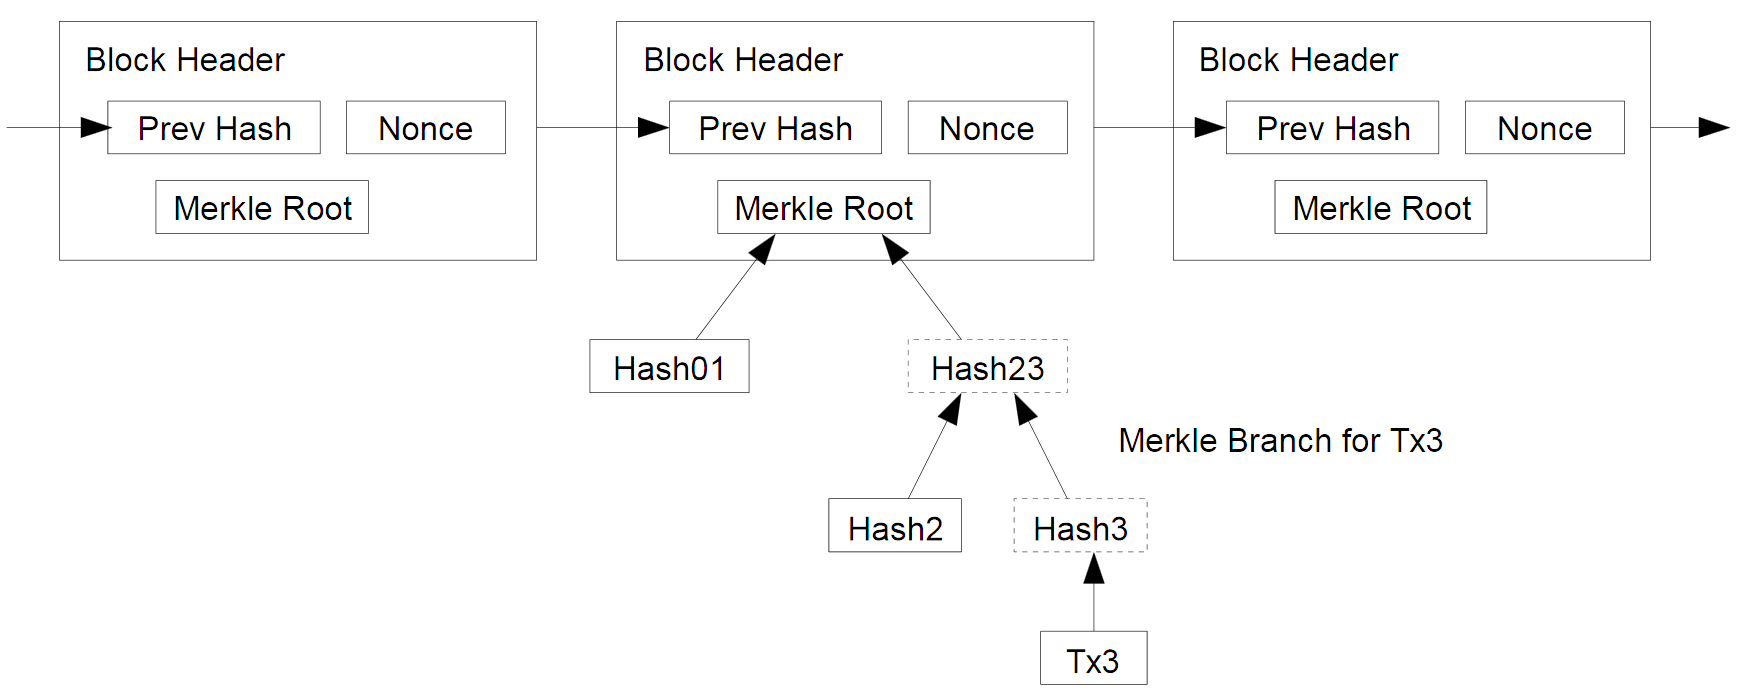
\includegraphics[scale=0.26]{../img/block-chain.png}
            }

        \end{overlayarea}
    \end{frame}
    %--------------------------------End-----------------------------------


    %--------------------------------Frame---------------------------------
    \begin{frame}
        \frametitle{What is a Blockchain?}

        \begin{overlayarea}{\textwidth}{\textheight}

            \vspace{4ex}

            \only<1-> {
            \centering {\huge Cool! But why?}
            }

            \only<2-> {
            \vspace{4ex}
            \begin{itemize}
                \item \alert{Suppress} the necessity of trusted third-party (i.e. financial institutions and banks).
                \item Move trust from central authorities to decentralized secure protocol.
                \item Create an economical system not driven by central institutions.
                \item \alert{Empower} people.
                \item Enable almost \alert{immediate} transactions.
                \item Offer lower fees than traditional banking.
                \item Let people become their own bank.
            \end{itemize}

            }

        \end{overlayarea}
    \end{frame}
    %--------------------------------End-----------------------------------


    %--------------------------------Frame---------------------------------
    \begin{frame}
    \begin{overlayarea}{\textwidth}{0.9\textheight}
        \frametitle{A bit more background}

        \begin{itemize}
            \item Since Bitcoin appearance in 2009, several other \st{cryptocurrencies} emerged.
            \pause
            \item Currently most of them are based in some kind of Blockchain.
            \pause
            \item Blockchain provides a reliable infrastructure that provides \st{at least} 2 out of the 3 properties of \st{CIA triad}: \alert{integrity} and \alert{availability}.
        \end{itemize}

        \vspace{-1ex}
        \only<1-6> {
        \begin{exampleblock}{Integrity}<4-6>
            By the use of asymmetric cryptography the integrity of the data is guaranteed.
        \end{exampleblock}

        \begin{exampleblock}{Availability}<5-6>
            As a decentralized network, there is no single point of failure.
        \end{exampleblock}

        \begin{block}{Confidentiality}<6>
            It seems that some implementations could provide it as well (e.g.\ ZCash).
        \end{block}
        }

        \only<7-> {
            \vspace{3ex}
            \centering
            \begin{minipage}{0.7\textwidth}
            \begin{alertblock}{}
                \centering
                {\large \ts{`` We can see it as an Internet-native way to store and exchange value ''}}
            \end{alertblock}
            \end{minipage}
        }

    \end{overlayarea}
    \end{frame}
    %--------------------------------End-----------------------------------


    \section{How does it work?}
    \subsection{Consensus}
    %--------------------------------Frame---------------------------------
    \begin{frame}
        \frametitle{How does it work?}

        \begin{overlayarea}{\textwidth}{0.7\textheight}

            \only<1-> {
            \begin{center}
                \Huge \ts{``It is all about consensus''}
            \end{center}
            }

            \only<2-6> {
            \begin{itemize}
                \itemsep=1ex
                \pause
                \item Blockchain concept is in continuous \st{evolution} and new protocols are continuously created to improve the current flaws.
                \pause
                \item Earliest implementations (which includes Bitcoin and Ethereum) are using a system called \eh{Proof of Work} (\st{PoW}) to \alert{validate} the transactions.
                \pause
                \item \st{Validation} is required in order to append a new block of transactions to the chain; preventing things such as double spend.
                \pause
                \item The process of block validation is known as \st{mining}.
                \pause
                \item Lately a new system called \ts{Proof of Stake} (\st{PoS}) was developed to address PoW flaws.
            \end{itemize}
            }

            \only<7-> {
            \begin{itemize}
                \itemsep=1ex
                \item<7-> Nodes are motivated to maintain the network with a \st{reward} coming from transaction fees.
                \item<8-> Hence, \alert{consensus} is achieved though these systems (PoW/PoS).
            \end{itemize}
            }

        \end{overlayarea}
    \end{frame}
    %--------------------------------End-----------------------------------


    %--------------------------------Frame---------------------------------
    \begin{frame}
        \frametitle{Transaction work-flow}

        \begin{enumerate}
            \itemsep=4ex
            \item Clients create and \alert{sign} transactions (TX) using their private key, then they \st{broadcast} TX to the network.
            \item Network nodes (miners) receive transactions and store them in the so called \st{mempool}.
            \item Miners \alert{prioritize} transactions based on fees, \alert{validate} and \alert{put} them in a block.
            \item Once successfully created and \alert{verified} by the network, the block is finally \alert{appended} to the chain.
        \end{enumerate}

    \end{frame}
    %--------------------------------End-----------------------------------


    %--------------------------------Frame---------------------------------
    \begin{frame}
        \frametitle{}

        \begin{center}
            \huge But how does it work under the hood?
        \end{center}

    \end{frame}
    %--------------------------------End-----------------------------------


    \subsection{Proof of Work}
    %--------------------------------Frame---------------------------------
    \begin{frame}
        \frametitle{Proof of Work: The Bitcoin case}
        \begin{overlayarea}{\textwidth}{\textheight}

            \only<1-2> {
            \vspace{2ex}
            \begin{exampleblock}{Block creation (mining)}
                Participants of a Blockchain network put computational \alert{resources} to validate transactions by \alert{solving} the so called \st{cryptographic puzzles}.
            \end{exampleblock}
            }

            \only<2> {
            \begin{itemize}
                \itemsep=1ex
                \item Block validation consists in finding a \st{nonce} (number) for the block that \st{satisfies} a property of the block's hash (a number of leading zeros) known as difficulty.
                \item This is a trial and error procedure (a kind of brute-force).
                \item The first node that finds a successful solution \st{announces} it to the network.
                \item The rest of the nodes can \alert{easily verify} that the solution (and hence the block) is valid.
                \item If a node acts \alert{dishonestly}, the rest of nodes will discard the block.
            \end{itemize}
            }

            %    \visible<3> {
            %        \begin{block}{How?}
            %            Taking the solution (nonce) into the block and computing block's hash (SHA-256) must result in a hash with a leading number of zeroes.\\
            %            This is easy to verify for any node.
            %        \end{block}
            %    }

            % Drawbacks
            \only<3> {
            \vspace{2ex}
            \begin{alertblock}{Drawbacks}
                \begin{itemize}
                    \item Huge energy consumption.
                    \item Susceptible to a 51\% attack.
                    \item Democratization of the network (hardware, electricity price,\ldots)
                \end{itemize}
            \end{alertblock}
            }

        \end{overlayarea}
    \end{frame}
    %--------------------------------End-----------------------------------


    \subsection{Proof of Stake}
    %--------------------------------Frame---------------------------------
    \begin{frame}
        \frametitle{Proof of Stake}
        \begin{overlayarea}{\textwidth}{0.85\textheight}

            \only<1-2> {
            Given the aforementioned problems that PoW presents, the new Proof of Stake (PoS) model was developed.

            \begin{exampleblock}{Block creation (forging)}
                Participants of the network \alert{stake} an amount of currency they hold (a kind of deposit) to be able to forge and \alert{send} a block to the network.
            \end{exampleblock}
            }

            \only<2> {
            \begin{itemize}
                \item The next block creator (called forger) will be chosen randomly following certain criteria.
                \item The forger \st{verifies} transactions, \st{forges} a new block and \st{sends} it to the network.
                \item As in PoW, new block is added to the chain and forger receives transaction fees (and its stake back).
                \item If the forger acts \alert{dishonestly}, the rest of nodes will discard the block and forger will \alert{lose} the \st{stake}.
            \end{itemize}
            }

            \only<3> {
            \begin{exampleblock}{Pros}
                \begin{itemize}
                    \item A way more \st{energy} efficient: there are no computational resources required.
                    \item More democratization and hence \st{decentralization}.
                    \item \st{Security}: Purchasing more than half of the coins is likely more costly than acquiring 51\% of PoS hashing power.
                \end{itemize}
            \end{exampleblock}

            \begin{alertblock}{}
                Several proposals have been presented, studied and even implemented but PoS still faces some \alert{challenges} that must be addressed.
            \end{alertblock}

            }

            \only<4> {
            \vspace{2mm}
            \centering
            {\huge \sl{`` Not so \alert{trivial} ''}}

            \vspace{3ex}
            \begin{columns}[c]
                \column{0.5\textwidth}
                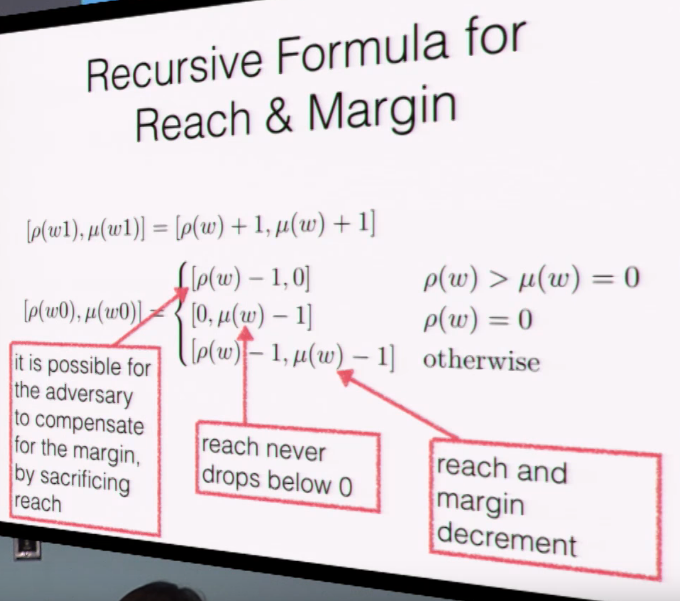
\includegraphics[scale=0.245]{../img/ouroboros-1.png}

                \column{0.5\textwidth}
                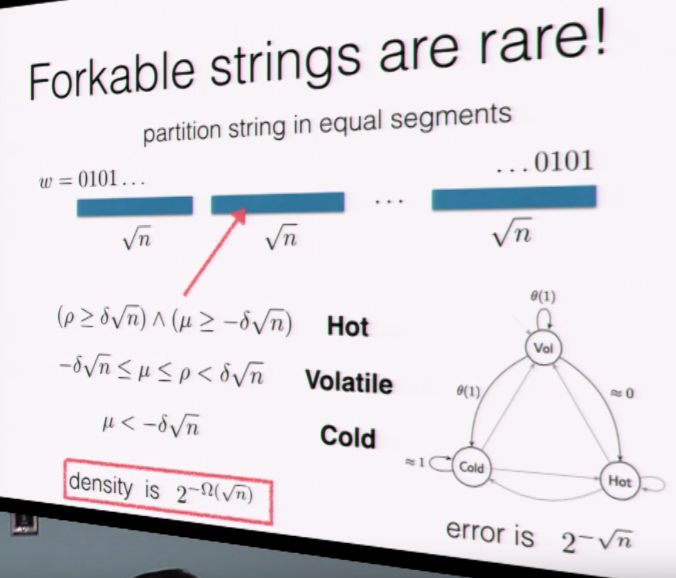
\includegraphics[scale=0.255]{../img/ouroboros-2.png}
            \end{columns}
            \vspace{1ex}
            {\footnotesize Ouroboros: A Provably Secure Proof-of-Stake Blockchain Protocol}}

        \end{overlayarea}
    \end{frame}
    %--------------------------------End-----------------------------------


    \section{Blockchain by generations}
    \subsection{Preliminaries}
    %--------------------------------Frame---------------------------------
    \begin{frame}
        \frametitle{Definition}

        \begin{block}{Turing Completeness}
            A programming language is said to be Turing Complete (TC) if can be used to simulate a Turing Machine and hence to \alert{solve any} mathematical/ computational problem.\\[2ex]
                        
            A TC-language has some important \st{properties}:
            \begin{itemize}
                \item conditional branching;
                \item infinite \textbf{looping} ability;
                \item $[$\ldots$]$
            \end{itemize}
        \end{block}

    \end{frame}
    %--------------------------------End-----------------------------------
    
    
    \subsection{First Generation}
    %--------------------------------Frame---------------------------------
    \begin{frame}
        \frametitle{First Generation: Bitcoin}
        
        Bitcoin was the first implementation of the Blockchain and is considered the \st{first generation} of Blockchain.

        \begin{columns}
            \column{0.75\textwidth}
                \begin{itemize}\itemsep=1.35ex
                    \item Bitcoin has a programming language called \textbf{Script} used to ``encode'' the transactions, and to \st{control} how the payee of a TX can access the funds.
                    \item But, Script is \alert{not} a \textbf{TC-language} (has no loops)\ldots
                    \item \ldots so Bitcoin can be \st{merely} used as a \alert{store of value} and \alert{exchange of value} network.
                \end{itemize}       
                
            \column{0.25\textwidth}
            
\includegraphics[scale=0.25]{../img/anonymous.png}
        \end{columns}

        \vspace{1ex}
        \begin{exampleblock}{}<2->
            For its nature, it is usually called digital gold.
        \end{exampleblock}

        \begin{alertblock}{}<3->
            \textbf{Current} implementation presents \alert{scalability} issues ($\approx$ 7 TPS)
        \end{alertblock}

        
    \end{frame}
    %--------------------------------End-----------------------------------


    \subsection{Second Generation}
    %--------------------------------Frame---------------------------------
    \begin{frame}
    \begin{overlayarea}{\textwidth}{0.8\textheight}    
        \frametitle{Second Generation: Ethereum}
        
        Ethereum, which is considered a \st{second generation Blockchain}, was released in 2015 after two years of research and development.

        \begin{columns}
        
            \column{0.74\textwidth}
            \begin{itemize}\itemsep=0.4ex
                \item Co-founded by Vitalik Buterin, a young cryptocurrency researcher/programmer.
                \item Features a \textbf{TC-complete} programming language called \textbf{Solidity} {\footnotesize(and experimental Vyper)}.
                \item An \st{abstraction} of the 1st gen. that allows \alert{not only} exchange ``money'' but the execution of any program.
                \item These programs are called \st{Smart Contracts}.
                \item Users pay fees for contract (program) execution.
            \end{itemize}
                    
            \column{0.26\textwidth}
            \centering
            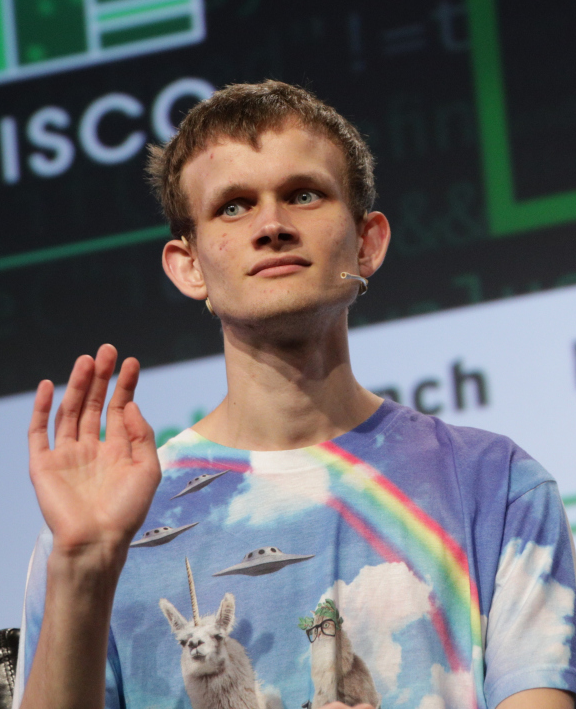
\includegraphics[scale=0.15]{../img/vitalik.png}\\
            {\scriptsize Vitalik Buterin}
        \end{columns}
        
        \begin{exampleblock}{}<2->
            Ethereum is in essence a \st{decentralized application network}
        \end{exampleblock}
        
        \vspace{-1.2ex}
        \begin{alertblock}{}<3->
            \textbf{Current} implementation presents \alert{scalability} issues ($\approx$ 15 TPS) 
        \end{alertblock}

    \end{overlayarea}    
    \end{frame}
    %--------------------------------End-----------------------------------


    %--------------------------------Frame---------------------------------
    \begin{frame}
        \frametitle{Smart Contracts}
        
        \begin{center}
        \begin{minipage}{0.75\textwidth}
        \begin{quote}<1->
            ``A smart contract is a set of promises, specified in digital form, including protocols within which the parties perform on these promises.''
            \vspace{-.5ex}
            \flushright {\small Nick Szabo, 1996}
        \end{quote}
        \end{minipage}
        \end{center}

        \begin{exampleblock}{Example: ICO}<2->
            When participating in an Initial Coin Offer (ICO) a user \alert{sends funds} (an investment) to a Smart Contract.\\[2ex]

            The contract \alert{encodes the rules} of the agreement: usually a number of tokens proportional to the investment will be
            sent back to the user (which represents his investment in the project).\\[2ex]

            \alert{No third party} is involved.
        \end{exampleblock}


    \end{frame}
    %--------------------------------End-----------------------------------


    \subsection{Third Generation}
    %--------------------------------Frame---------------------------------
    \begin{frame}
    \begin{overlayarea}{\textwidth}{0.75\textheight}
        \frametitle{Third Generation}

        The 3rd generation of Blockchain is mainly focused to \st{address} two of the main issues of the 2nd generation:
    
        \vspace{1ex}
    
        \only<1-3> {
            \begin{itemize}
                \item Scalability
                \item Security
            \end{itemize}

        

            \begin{block}{Scalability}<2->
                A 3rd generation of Blockchain should be able to scale to \st{several thousands} of TPS.\\[1ex]
                
                Network usage (\st{bandwidth}) and \st{data} storage should scale efficiently.
            \end{block}
            
            \begin{block}{Security}<3->
                Smart contracts should be able to be verified using \st{Formal Verification}.
            \end{block}
        }

        \only<4-> {

            \begin{columns}

                \column{0.42\textwidth}
                \begin{exampleblock}{Cardano}
                    is a 3rd generation Blockchain focused to address limitations of 2nd generation Blockchains.
                \end{exampleblock}

                \column{0.45\textwidth}
                \centering
                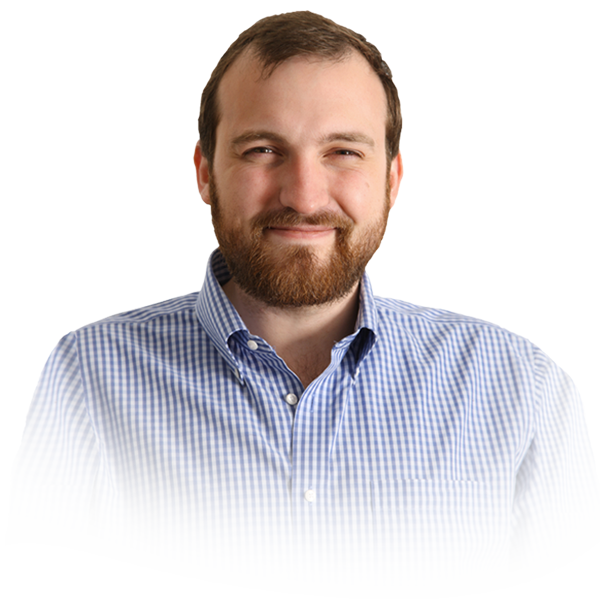
\includegraphics[scale=0.15]{../img/hoskinson.png}\\
                {\scriptsize Charles Hoskinson,\\ co-founder of Cardano\\[-1ex] and former co-founder of Ethereum}

            \end{columns}
        }
    \end{overlayarea}
    \end{frame}
    %--------------------------------End-----------------------------------


    \section{Cardano: A scientific research-driven Blockchain}
    %--------------------------------Frame---------------------------------
    \begin{frame}
        \frametitle{Cardano}

        \centering
        
\includegraphics[scale=0.07]{../img/cardano.png}

        \begin{itemize}
            \itemsep=1.35ex
            \item Born in 2015 as an effort to \st{change the way} cryptocurrencies are designed and developed.
            \item Developed together by IOHK company and several universities.
            \item \st{Scientific} research \st{model} and \alert{peer review}.
            \item The Blockchain for ADA cryptocurrency.
            \item Considered a \alert{3rd generation} Blockchain.
            \item Different approach: \alert{How to scale} instead of how many TPS.
            \item Current development roadmap planned at least until 2020.
            \item ADA was launched to trade in October 2017.
        \end{itemize}


    \end{frame}
    %--------------------------------End-----------------------------------


    %--------------------------------Frame---------------------------------
    \begin{frame}
        \frametitle{Cardano}

        \begin{exampleblock}{Key features}
            \begin{itemize}
                \item \st{Proof of Stake} (Ouroboros consensus algorithm)
                \item \st{Sustainable} ecosystem
                \item Strongly focused on \st{scalability}
                \item \st{Interoperability} with other Blockchains
                \item Smart contracts
                \item Treasury
                \item Based on \st{epochs} and \st{quorums}
                \item \st{Parallelize} transactions amongst quorums will allow to \alert{scale}
                \item Reduces network \st{pressure} by using RINA
            \end{itemize}
        \end{exampleblock}

    \end{frame}
    %--------------------------------End-----------------------------------


    %--------------------------------Frame---------------------------------
    \begin{frame}
        \frametitle{Cardano}
        \begin{overlayarea}{\textwidth}{0.8\textheight}

            \only<1-> {
            Aims to \alert{solve} 3 main problems of current cryptocurrencies:
            \begin{itemize}
                \item Scalability
                \item Interoperability
                \item Sustainability
            \end{itemize}
            }

            \only<2> {
            \begin{block}{Scalability}

                \begin{tabular}{lcl}
                    \st{PoS} and  \st{parallelization} of epochs &  $\longrightarrow$ &  $\Delta$ TPS {\footnotesize (Transactions per second)} \\[1ex]
                    Split network in \st{subnets} (RINA)         &  $\longrightarrow$ &  $\nabla$ Bandwidth \\[1ex]
                    Pruning, compression, partitioning &  $\longrightarrow$ &  $\nabla$ Storage \\[1ex]

                \end{tabular}

            \end{block}
            }

            \only<3> {
            \begin{block}{Interoperability}
                Allow different cryptocurrencies to \st{talk each other}.\\[1ex]

                Allows \st{metadata} into TX $\longrightarrow$ Better integration with banks/governments.\\[1ex]

            \end{block}
            }

            \only<4> {
            \begin{block}{Sustainability (Treasury)}
                
                The \st{treasury} is a special wallet not controlled by anyone that receives a small percentage of every transaction.\\[1ex]
                
                It promotes \st{continuous improvement} of the system by funding the most voted improvement proposals.\\[1ex]
                    
                It will keep Cardano sustainable.\\[1ex]
                
                Powered by smart contracts.\\[1ex]
            \end{block}
            }

        \end{overlayarea}
    \end{frame}
    %--------------------------------End-----------------------------------

    \section{Cryptocurrency wallets}
    %--------------------------------Frame---------------------------------
    \begin{frame}
        \frametitle{Cryptocurrency wallets}

        % TODO
        TODO - Work in progress...
        % Blockchain: Don't need to trust anyone but yourself.
        % Drawback? Key lost = irrecoverable funds



    \end{frame}
    %--------------------------------End-----------------------------------


    \section{Why is it revolutionary?}
    \subsection{The future is decentralized}
    %--------------------------------Frame---------------------------------
    \begin{frame}
        \frametitle{The future is decentralized}

        \visible<1-> {
            Since its creation, Internet has been \st{mostly} centralized\footnote{ARPANET hosts file is a great example.},
            which implies that it is:

            \vspace{-1ex}
            \begin{itemize}
                \item Easy to \alert{watch/monitor}
                \item Easy to \alert{censor}
                \item Easy to \alert{attack}
                \item \alert{Fragile} to failure
            \end{itemize}

            During the years more distributed and P2P protocols has been deployed, but client-server model is the most common yet.
        }

        \vspace{1ex}
        \visible<2-> {
            \begin{exampleblock}{}
                But the appearance of new P2P systems can drive Internet to a new state
            \end{exampleblock}
        }

    \end{frame}
    %--------------------------------End-----------------------------------


    %--------------------------------Frame---------------------------------
    \begin{frame}
        \frametitle{The future is decentralized}

        \only<1> {
            \centering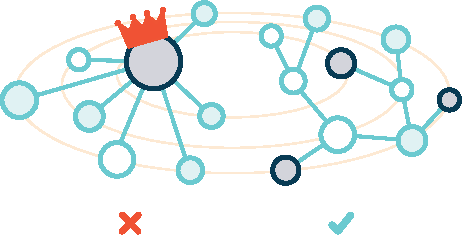
\includegraphics[scale=0.5]{../img/ipfs.pdf}

            \begin{exampleblock}{A nice example}
                \href{https://ipfs.io/}{IPFS} (Inter Planetary File System)
            \end{exampleblock}

            \begin{exampleblock}{Another example}
                \href{https://steemit.com/}{Steemit} is a blogging/social media website built on top of a \st{Blockchain}.\\[1ex]

                Steemit has proven to be able to run an entire social network in a Blockchain.\\[1ex]

                All blog entries are stored in the Blockchain.
            \end{exampleblock}
        }

        \only<2> {
            \vspace{-2em}
            \begin{center}{\huge The future of the Internet?}\end{center}

            \vspace{2em}
            \begin{columns}
                \column{0.65\textwidth}
                \centering
                \begin{minipage}{5cm}
                \begin{block}{Decentralization provides}
                    \begin{itemize}
                        \item censorship resistance
                        \item freedom of Internet
                        \item democratization
                        \item more privacy
                    \end{itemize}
                \end{block}
                \end{minipage}

                \column{0.35\textwidth}
                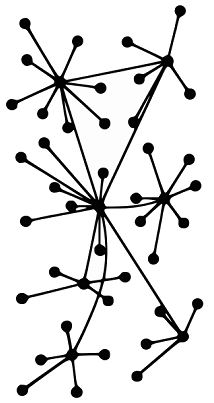
\includegraphics[scale=0.3]{../img/decentralization.png}
            \end{columns}
        }

    \end{frame}
    %--------------------------------End-----------------------------------


    \subsection{Worldwide financial services}
    %--------------------------------Frame---------------------------------
    \begin{frame}
    \begin{overlayarea}{\textwidth}{0.9\textheight}
        \frametitle{Worldwide financial services}

        \only<1-2> {
        \vspace{1em}
        \begin{itemize}
            \itemsep=1.5ex
            \item $>$50\% of world's population ({\footnotesize 2-3 billion people}) does \alert{not have access} to formal, or any kind of financial services at all.
            \item People \st{sending money} to their families in developing or third world countries pay \alert{very high} fees.
            \item Access to \st{loans} for those unbanked collectives is difficult and they pay \alert{extraordinary high} interests ({\footnotesize $>$100\% in some cases}).
        \end{itemize}

            \only<2-> {
                \begin{exampleblock}{}
                    Blockchain and Smart Contracts could provide the infrastructure to tackle such a serious problem.
                \end{exampleblock}
            }
        }

        \only<3> {
                \vspace{0.5ex}
                \centering
                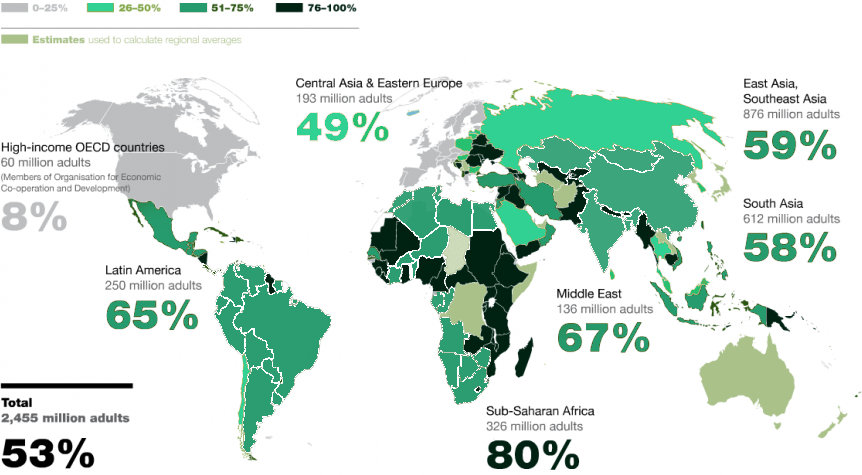
\includegraphics[scale=0.5]{../img/worlds-nonfinancial-population.png}\\[2ex]
                Percentage of unbanked people. {\footnotesize Source: \href{https://ethichub.com}{ethichub.com}}.
        }

        \only<4> {
            \vspace{0.5ex}
            \centering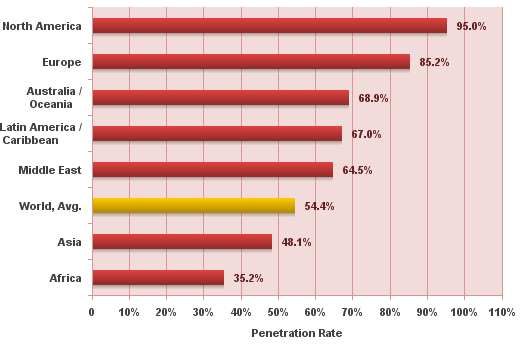
\includegraphics[scale=0.45]{../img/internet-penetration.png}

            \vspace{-0.5ex}
            \begin{alertblock}{But\ldots}
                Only 54.4\% of world's population have access to Internet ({\footnotesize Internet World Stats 2018}).
            \end{alertblock}
        }

    \end{overlayarea}
    \end{frame}
    %--------------------------------End-----------------------------------


    %--------------------------------Frame---------------------------------
    \begin{frame}
        \frametitle{Technology to the rescue again}

        \begin{columns}
            \column{0.65\textwidth}

            \only<1> {
                \begin{itemize}
                    \itemsep=1.5ex
                    \item \st{\textbf{Starlink}} is a project of SpaceX and co-financed by Google that aims to provide a global Internet connection using a constellation of satellites.
                    \item Recently the first two satellites of what aims to conform a worldwide-available hi-speed Internet network have been launched.
                    \item In near future, it could \alert{potentially provide} Internet access to hundreds of millions of people that are offline nowadays.
                \end{itemize}
            }

            \only<2> {
                \begin{itemize}
                    \itemsep=1.5ex
                    \item The combination of all these could \alert{empower people}, bringing financial services everywhere.
                    \item Everyone could become its own bank.
                    \item Think about yourself being able to crediting third world population.
                    \item It could flip the whole system.
                \end{itemize}
            }

            \column{0.35\textwidth}
            \centering
            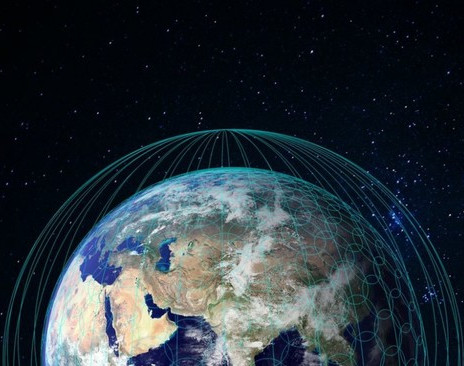
\includegraphics[scale=0.247]{../img/starlink.jpg} \\[1ex]
            {\Large +} \\[1ex]
            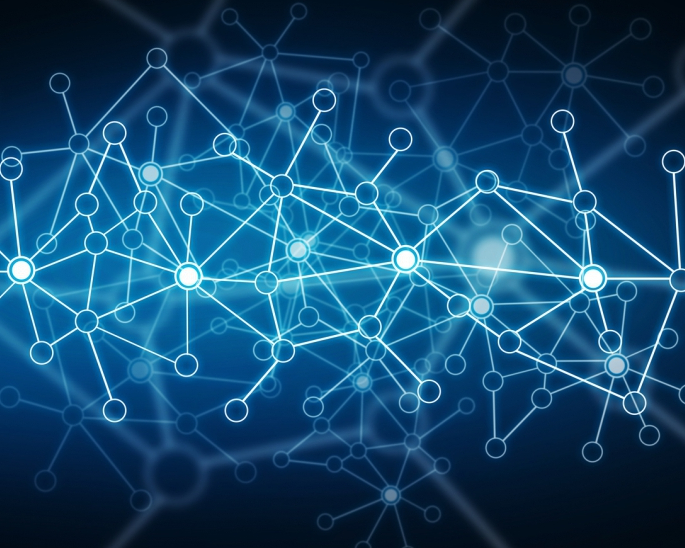
\includegraphics[scale=0.17]{../img/blockchain-fancy.jpg}

        \end{columns}


    \end{frame}
    %--------------------------------End-----------------------------------


    \section{Some conclusions}
    %--------------------------------Frame---------------------------------
    \begin{frame}
        \frametitle{Some conclusions}

        As a result of all these, one can think:

        \begin{itemize}
            \itemsep=1.35ex
            \item Wow! Technology is always awesome and has power to change the world.
            \item \st{Traditional} financial model is becoming out-dated\ldots
            \item \ldots but for now, Blockchain ecosystem is probably \st{not yet} mature enough to drive world's economy.
            \item The future is going to be more decentralized.
            \item Awesome things could happen, but only \alert{time will tell}.
        \end{itemize}

    \end{frame}
    %--------------------------------End-----------------------------------

    \section*{}
    %--------------------------------Frame---------------------------------
    \begin{frame}
        \frametitle{}
        
        \centering
        \Huge Thanks for your time! \\[2ex]
        
        \huge Questions?

    \end{frame}
    %--------------------------------End-----------------------------------
    

    %--------------------------------Frame---------------------------------
    \begin{frame}
        \frametitle{License}

        These slides are licensed under Creative Commons CC-BY-NC-SA.

        \begin{center}
\includegraphics[scale=0.6]{../img/cc-by-nc-sa.png}\end{center}
        
        \vspace{2ex}
        \begin{columns}
            \column{0.47\textwidth}
            \centering
            Slides code available on GitHub: \\[1ex]
            
\includegraphics[scale=0.06]{../img/github-repo.png} \\
            \tiny \href{https://github.com/gerardbosch/blockchain-presentation}{github.com/gerardbosch/blockchain-presentation}
        
            \column{0.49\textwidth}
            \centering
            Updated PDF available online: \\
            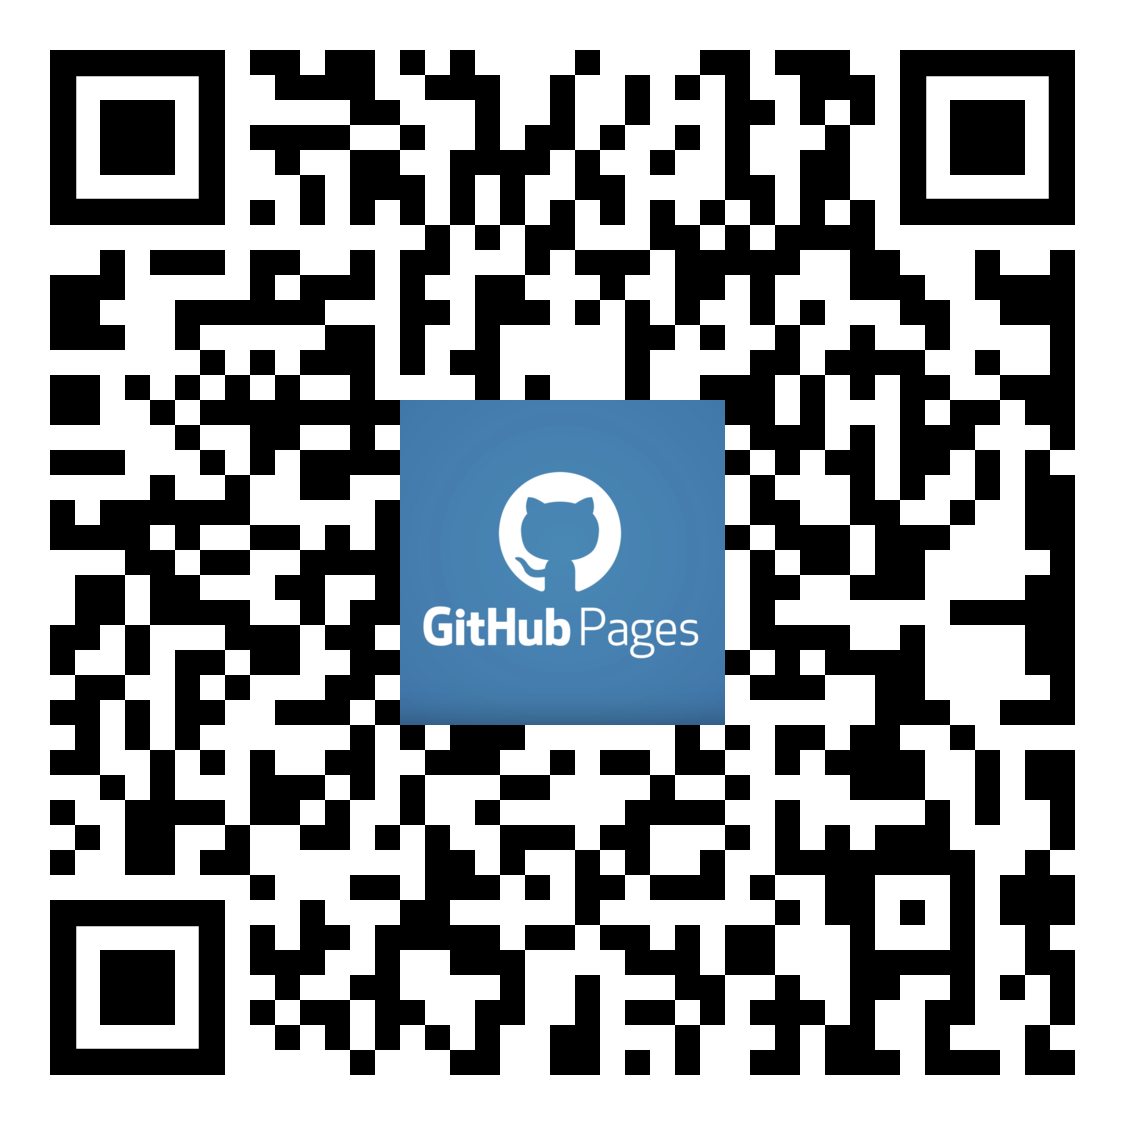
\includegraphics[scale=0.06]{../img/online-pdf-qr.png} \\
            \tiny \href{https://gerardbosch.github.io/blockchain-presentation/}{gerardbosch.github.io/blockchain-presentation}
        
        \end{columns}


    \end{frame}
    %--------------------------------End-----------------------------------


\end{document}


%--------------------------------Frame---------------------------------
\begin{frame}
    \frametitle{}

\end{frame}
%--------------------------------End-----------------------------------
